\section{Methods \label{sec:methods}}

To archive clustering, the method adopted was to compare document using the authorship linkings strategies presented in \textit{Evaluation of text representation schemes and distance measures for authorship linking}~\cite{kocher_verification}.
These method aim to compare the simlarity of documents by considering reccurent stylistic patterns.
Text patterns can be for example from either reccurant words or Part-Of-Speech (POS).
Another possible way compare similarities between document explored in this study is to use compression techniques.

To archive a good clustering, the main objective is to have the most reliable authorship linking rank list possible.
To increase the quality of the rank list, the proposed method is to use a combination of multiple rank list using different strategies to form an optimistically better rank list.
By using the most diverse strategies, we believe it is possible to increase the quality using the principle of combination of evidences.

\subsection{Most frequant words (MFW), feature vectors}

The first method used is called: Most frequant words (acronym: MFW), and try to compare the documents by creating feature vectors containing words frequencies.
To be able to express a document as a feature vector of size $n$, a common strategy in Stylometry is to find the $n$ most frequent words ($n$-MFW) in a corpus, and for each document compute the relative frequency of each of these words for the document~\cite{savoy_stylo}.
For example if the word : "\textit{the}" is in the $n$-MFW and occurs $50$ times in a document with $300$ words, its relative frequency is thus $50/300 = 1/6$, the word and the value will be in the feature vector if the frequency is in the top $n$-MFW.
No clear value of $n$ for the $n$-MFW is to choose over others, but a value between $50$ and $500$ tends to produce good results for the word token text representation~\cite{savoy_text_representation}.

Instead of using directly the words to create the feature vector, another possibility is to use the lemma corresponding to each word, for example the sentence \textit{I saw two men with a saw} its lemmatized version is : \textit{I see two man with a saw} this requires advanced text preprocessing, but it can remove ambiguity.

Another popular method is instead of considering every token as a word, this method aim to create a "word" from a short sequences of letters called $n$-grams using Definition~\ref{def:letters_n_grams}.
To consider an overlapping word, the whole document is synthesized into a long string by joining every token by an \textit{underscore} : $\_$.
This technique can be further exploited by combining for example two or more sizes of $n$-grams together.
$n$-grams can be really effective even though no clear meaning from each $n$-grams can be exploited at first sight.
A simple explaination of why $n$-grams can be effective is by using $n$-grams of size 3 to 5 in most germanic languages this can correspond to for example : the tense of the verbs (i.e. : \textit{ing\_}, \textit{ed\_}), some small common words (\textit{\_the\_}, \textit{\_and\_}, \textit{\_that}), or in French the adverbs (\textit{\_ment}), etc.

\begin{definition}[Letters $n$-grams]
  \label{def:letters_n_grams}
  A letter $n$-grams is a special type of tokenization which is constructed by creating a token of size $n$ for each substrings starting from the position $0$ to \textit{text\_size} $- n - 1$.
  Example: Using 3-grams The string: \textit{"fox\_is\_brown"} is converted to: (\textit{"fox", "ox\_", "x\_i", "\_is", "is\_", "s\_b", "\_br", "bro", "row", "own"})
\end{definition}

An alternative version of the $n$-grams algorithm used here is defined in~Definition~\ref{def:words_n_grams}.
This algorithm consider each token as a string to apply the Letters $n$-grams algorithm to.
To differenciate it from the classical $n$-grams algorithm,
The latter algorithm, is called in this study In-word $n$-grams (Definition~\ref{def:words_n_grams}) and the other one is  called Letters $n$-grams (Definition~\ref{def:letters_n_grams}).

\begin{definition}[In-words $n$-grams]
  \label{def:words_n_grams}
  In-word $n$-grams are created by applying the Letters $n$-grams algorithm on a each tokens.
  When a token is smaller than $n$, the whole token is considered.
  Example: Using words 3-grams on following tokens: ["fox", "is", "brown"] is converted to: (\textit{"fox", "is", "bro", "row, "own"})
\end{definition}

Another possible stylistic aspect that can be detected from a text using the MFW approach is to consider the sentence constructions.
This can be solved by creating short sequences ($n$-grams) of POS tags.
In this case, each POS is considered as a character in the Letters $n$-grams definition, this type of $n$-grams is also known as w-shingling.
For example, the sentence : \textit{"The cat eat a fish"} has the following POS tag \textit{"Article Noun Verb Article Noun"} which correspond to the following 3-grams of POS : \textit{"Article Noun Verb"} / \textit{"Noun Verb Article"} / \textit{"Verb Article Noun"}.
In practice the POS is more detailed, for example instead of just considering \textit{eat} as a verb, a more detailed POS can be the verb and its tense \textit{Verb-SimplePresent}, the same goes for the other type of POS.

When using features vectors based on the MFW approaches, once each document is represented as a feature vector they can be compared using metric in Section~\ref{sec:fv_distances}.

\subsubsection{Vectors distances}
\label{sec:fv_distances}

To be able to compare vector, different metrics can be used depending on the usage.
Usually two types of metrics for vector comparison can be used: Vector similarities and Vector distances, the first yield a large value when the two vectors are closely related and the second a small value when they are similar.
The following definitions are one of the few most common $L^1$/$L^2$/$cosine$ based distances.

\begin{definition}[Manhattan distance ($L^1$ based)]
  To compute the Manhattan distance the following formula is used.
  \begin{equation}
    dist_{Manhattan}(A, B) = \sum_{i=1}^{m} |A_i - B_i|
  \end{equation}
\end{definition}

\begin{definition}[Tanimoto distance ($L^1$ based, normalized)]
  To compute the Tanimoto distance the following formula is used.
  It's a components-wised normalized version of the manhattan distance.
  \begin{equation}
    dist_{Tanimoto}(A, B) = \frac{dist_{Manhattan}(A, B)}{\sum_{i=1}^{m} max(A_i, B_i)}
  \end{equation}
\end{definition}

\begin{definition}[Euclidean distance ($L^2$ based)]
  To compute the Euclidean distance the following formula is used.
  \begin{equation}
    dist_{Euclidian}(A, B) = \sqrt{\sum_{i=0}^{m}(A_i - B_i)^2}
  \end{equation}
\end{definition}

\begin{definition}[Matusita distance ($L^2$ based, square rooted values)]
  To compute the Matusita distance the following formula is used.
  \begin{equation}
    \begin{split}
      dist_{Matusita}(A, B) &= dist_{Euclidian}(A', B') \\
      \text{with }A' &= \sqrt{A}\text{ and }B' = \sqrt{B}
    \end{split}
  \end{equation}
\end{definition}

\begin{definition}[Clark distance ($L^2$ based)~\cite{kocher_verification}]
  To compute the Clark distance the following formula is used.
  \begin{equation}
    dist_{Clark}(A, B) = \sqrt{\sum_{i=0}^{m}\left(\frac{|A_i - B_i|}{A_i + B_i}\right)^2}
  \end{equation}
\end{definition}

\begin{definition}[Cosine distance (Inner product based)]
  \label{def:cosine_dist}
  To compute the Cosine distance, first the cosine similarity must be computed.
  \begin{equation}
    sim_{Cosine}(A, B) = \frac{A \cdot B}{\sqrt{A \cdot A}\sqrt{B \cdot B}}
  \end{equation}
  The cosine similarity is ranged between -1 and 1.
  With 1 beeing exactly the same, -1 the total opposite and 0 orthogonal.
  \begin{equation}
    dist_{Cosine}(A, B) = 1 - sim_{Cosine}(A, B)
  \end{equation}
  \begin{equation}
    dist_{Angular\ cosine}(A, B) = \frac{cos^{-1}sim_{Cosine}(A, B)}{\pi}
  \end{equation}
\end{definition}

\begin{definition}[Kullback-Leibler divergence (relative entropy)]
  To compute the Kullback-Leibler divergence the formula below is used.
  \begin{equation}
    dist_{kld}(A, B) = \sum_{i=0}^{m} A_i \cdot \log(\frac{A_i}{B_i})
  \end{equation}
\end{definition}

\begin{definition}[Jeffrey divergence~\cite{kocher_verification}]
  To compute the Jeffrey divergence the formula below is used.
  It represents the difference between two probability distribution.
  \begin{equation}
    dist_{j\_divergence}(A, B) = \sum_{i=0}^{m} (A_i - B_i) \cdot \log(\frac{A_i}{B_i})
  \end{equation}
\end{definition}


\subsubsection{Normalization}

Sometimes when vectors deal with different order of magnitude, they can be not easily compared with some previously cited distance metrics.
Thus using a normalization can make the task easier.

\begin{definition}[Z-score normalization~\cite{savoy_stylo}]
  \label{def:z_score}
  \begin{equation}
    Zscore(A) = \frac{A - \mu}{\sigma}
  \end{equation}
  When using the z-score normalization on MFW vectors, $\mu$ and $\sigma$ usually are vectors containing the mean and the standard deviation of each terms in the corpus.
\end{definition}

The Manhattan distance applied on a Z-score normalized MFW vector is also called Burrows's Delta~\cite{savoy_stylo}.

\subsubsection{Smoothing}

Relative term frequencies can be considered as a probability of occurrence by using the maximum likelihood principle.
The main problem with this approach is that the probability of occurrence of frequent terms tend to be overhestimated and underestimate the probability of occurrence of low frequency terms.
If for example, a term is not present in a document its relative term frequency is 0, but this should not mean that the probability of the author using this word is 0.
The solution proposed is to use smoothing, such as the Lidstone smoothing presented in Definition~\ref{def:lidstone_smoothing}.
Smoothing techniques can help distance functions based on probabilities, such as the Kullback-Leibler Divergence.~\cite{savoy_stylo}

\begin{definition}[Lidstone smoothing~\cite{savoy_stylo}]
  \label{def:lidstone_smoothing}
  \begin{equation}
    p(t_i, D_j) = \frac{tf_{i,j} + \lambda}{n + \lambda \cdot |V|}
  \end{equation}
  With $t_i$ the i-th term, $D_j$ the j-th document, $tf_{i,j}$ the number of occurrence of the i-th term in $D_j$, $|V|$ the size of the vocabulary, $\lambda$ a small value ($\lambda = 1$ special, case called Laplace smoothing, but generally a smaller value such as 0.1 give good results), n the total number of words in the document $D_j$.
\end{definition}

In this study, when a smoothing technique is used, except stated otherwise, the Lidstone smoothing is used with $\lambda = 0.1$.

\subsection{Compression-based distances \label{sec:compression_based_distances}}

This section covers the compression based strategy to compute a distance between two documents.
The main idea is to compress two documents A, B, compress the string concatenation AB of A, B and compare their sizes after compression using one of the distance measure demonstrated below.
Commonly a lossless compression algorithm is used, such as the Lempel-Ziv family (GZIP), block sorting family (BZip2), statistical family (PPM)~\cite{comparing_compression}.
This technique is based on the fact that compression algorithms tries to lower the Shannon entropy of a document, thus when compressing a document with a large Shannon entropy the compressed document should have a larger size after compression than a document with a small Shannon entropy.
When concatenating two documents with a lot in common, the entropy of the concatenated document should be lower than if the two documents are very different.
This approach has the benefit can produce rank lists in a nearly parameterless manner, only a distance metric and compression algorithm is needed.
A main drawback with this technique is the fact that the results can not be properly explained.

In this study the lossless compression algorithm used are : GZip, BZip2, LZMA. These algorithm are already implemented in the python standard library~\cite{python_compression}.
Each compression algorithm can be tweaked with different parameters, the default settings are used except for the compression level (trade-off compression time and compression size).
By setting the compression level to the maximal setting, this ensure that the produced file will have the lowest possible Shannon entropy reachable with this algorithm, thus providing the best possible approximation of distance when used with the compression distances.

\begin{definition}[Conditional complexity of compression~\cite{savoy_stylo}~\cite{comparing_compression}]
  The conditional complexity of compression of two documents A and B using the size after compression C is computed as follow:
  \begin{equation}
    CCC(A, B) = C(AB) - C(A)
  \end{equation}
  This metrics is not easy to use since the order of magnitude is not bounded and can depend a lot on the text sizes.
  The following ones try to mitigate this problem.
\end{definition}

\begin{definition}[Normalized compression distance~\cite{savoy_stylo}~\cite{comparing_compression}]
  The normalized compression distance of two documents A and B using the size after compression C is computed as follow:
  \begin{equation}
    NCD(A, B) = \frac{C(AB) - \min(C(A), C(B))}{\max(C(A), C(B))}
  \end{equation}
  This metric gives a value in the range $\left[0, 1+\epsilon\right]$, with $\epsilon$ being a small positive value created by the imperfection of compression algorithms.
\end{definition}

\begin{definition}[Compression-based cosine~\cite{savoy_stylo}~\cite{comparing_compression}]
  The compression-based cosine of two documents A and B using the size after compression C is computed as follow:
  \begin{equation}
    CBC(A, B) = 1 - \frac{C(A) + C(B) - C(AB)}{\sqrt{C(A) \cdot C(B)}}
  \end{equation}
  This metric have the same properties as the cosine distance (Definition~\ref{def:cosine_dist}).
\end{definition}

\subsection{Rank lists}

Rank lists are used to order objects such that the most interesting object is at the top and every subsequent object become less interesting.
In information retrival systems, rank lists are used to order the results from the most relevant to the user's query to the least relevant.

\begin{definition}[Ranked list for authorship verification]
  A ranked list is a ordered list containing pairs of document.
  In most cases, the rank list contain every possible pairs of documents (every links).
  The ranked list is generally ordered by a score which can be either be ascendant in the case of scoring based on distance metrics and descendant when using similarity metrics.
  \begin{equation}
    L = (((X_a, X_b), Score(X_a, X_b)) | X_a \neq X_b \forall (X_a, X_b))
  \end{equation}
  \begin{equation}
    |L| = \frac{N \cdot (N - 1)}{2}
  \end{equation}
\end{definition}

\subsection{Rank list fusion}
\label{sec:rank_list_fusion}

The idea of rank list fusion is to combine multiple rank lists in such way that the resulting rank list is more accurate modelization of the real rank list.
The hypotetical best possible approximation of the real rank list in the case of authorship clustering is one such that  every true links (same authors document pairs) are at the top and every false links (different author document pairs) are at the bottom, therefore maximizing every metrics in Section~\ref{sec:rl_eval}.

\subsubsection{Z-Score fusion}

To merge scored rank list with differents order of magnitude, a simple and rather effective approach is to normalize every rank lists scores using the z-score (See Definition~\ref{def:z_score}) and then compute the merge rank list score for every link by taking the arithmetic mean of the same link score for every normalized rank lists.

\textbf{Example with the two rank lists:}

Rank list A (Mean = 50, Std = 40.82):

\begin{tabular}{c l r r}
  \toprule
  Rank & Link name & Score & Z-Score \\
  \midrule
  0 & (0, 1) & $100$ & $1.22$ \\
  1 & (1, 2) & $50$ & $0$ \\
  2 & (0, 2) & $0$ & $-1.22$ \\
  \bottomrule
\end{tabular}

Rank list B (Mean = 0.33, Std = 0.17):

\begin{tabular}{c l r r}
  \toprule
  Rank & Link name & Score & Z-Score \\
  \midrule
  0 & (1, 2) & $0.5$ & $0.98$ \\
  1 & (0, 1) & $0.4$ & $0.39$ \\
  2 & (0, 2) & $0.1$ & $-1.37$ \\
  \bottomrule
\end{tabular}

Z-Score fusion:

\begin{tabular}{c l l}
  \toprule
  Rank & Link name & Average Z-Score \\
  \midrule
  0 & (0, 1) & $(0.39 + 1.22) / 2$ = $0.81$ \\
  1 & (1, 2) & $(0 + 0.98) / 2$ = $0.49$ \\
  2 & (0, 2) & $(-1.22 + -1.37) / 2$ = $-1.30$ \\
  \bottomrule
\end{tabular}

This method can provide good results, but lack of theoretical foundations.

\subsubsection{Regression fusion}

Each rank list is ordered by a score, this score depends on distance measure used, thus the order of magnitude of each rank list is different.
To avoid having problems in merging rank lists with different magnitude, the solution opted is to translate the scores into a probability of being a true link.
To do so the logistic regression is used.
This method is similar to the one proposed in \textit{Anne Le Calvé and Jacques Savoy (2000)}'s paper~\cite{le_calve_database_merging} and used for merging rank list issued from information retrieval systems.

The main idea here is to learn a logistic regression model for each combination text representation and distance metrics used (here denoted \textit{type of rank list}).
The features used to find the logistic parameters for each link in the rank list are : the log of the relative rank and the link score.
Since a probability of being a true link is desired, the target value for each true link is 1 and 0 when it's a false link.

Once a model per type of rank list is trained, this model can provide for any new same type rank list, probabilities for each link being of being a true link.
The probability framework can now be used on the rank list.
To obtain the most reliable probability given multiple observations (different rank lists), the fusion result in computing the expected value for each link's probability using these observations.
In this case, the expected value is a simple average of the probabilities, since no weighting is used on the rank lists.

\subsubsection{Soft-veto using S-Curve}

An additional desired constraint is to favor top ranked link and penalize bottom ranked links when fusing rank lists.
This constraint can be easily explained by observing the distance over the rank graph of the rank list.
Figure~\ref{fig:distance_over_rank} clearly show us the top ranked links and bottom ranked links have a sharper decision than in than the middle section.

\begin{figure}
  \centering
  \caption{Distance over rank in the rank list using the smoothed Manhattan distance, 500 MFW tokens on the Brunet dataset}
  \label{fig:distance_over_rank}
  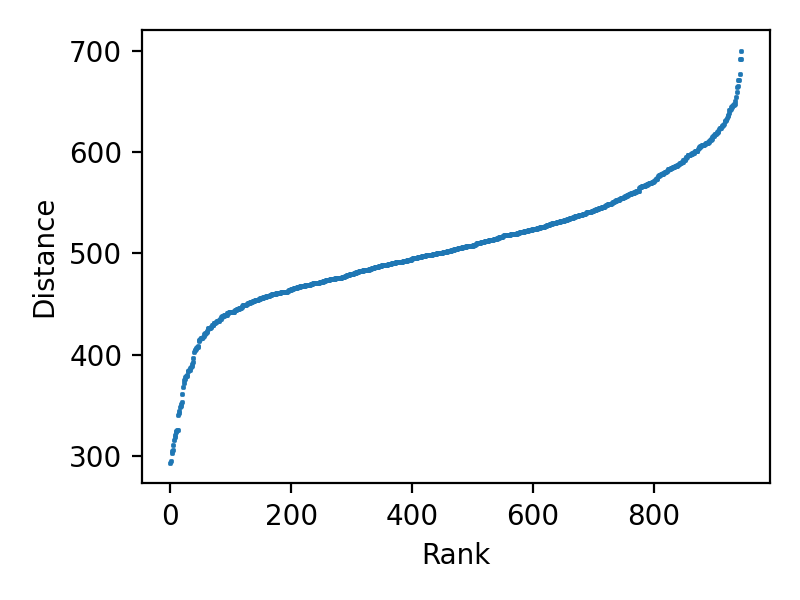
\includegraphics[width=\linewidth]{img/distance_over_rank.png}
\end{figure}

Top ranked links correspond to similar documents and bottom links correspond to negatively correlated documents.
Assuming that the top rank are true links after the rank list fusion these link should also be top rank.
The same reasoning can be apply for the bottom links by assuming them as false links.
A weighting curve, here called soft-veto, can be design accordingly such that top links are boosted and bottom links hindered.

Using the reciprocal of the sigmoid function such curve can modelized.

\begin{equation}
  \label{eq:sigmoid}
  S(x) = \frac{1}{1+e^{-x}}
\end{equation}
\begin{equation}
  \label{eq:sigmoid_r}
  S^{-1}(x) = -\ln{\frac{x-1}{x}}
\end{equation}

The steepness of the curve can be ajusted by changing the start and the end of the interval and then normalizing the values between 0 and 1.
Figure~\ref{fig:s_curve_c} shows the $S^-1(x)$ function normalized between -1 and 1 for the intervals between $\lim\limits_{c \rightarrow 0} \left[S(c), S(c)\right]$ and $\left[S(-20), S(+20)\right]$.
A greater interval size increase the steepness which correspond to an increase of the rank conservation of the top and bottom ranked links and decreasing the rank conservation of the middle ranked links.

To break the symmetry for the curve, to be able to increase the conservation of the top rank while decreasing the conservation of the bottom ranked.
The solution proposed is to take $r \cdot N$ samples for $\left[S(-c), S(0)\right]$ and $(1-r) \cdot N$ samples for $\left[S(0), S(c)\right]$.
Figure~\ref{fig:s_curve_r} shows the r parameter influance of a sigmoid with $c = 4$ and $r \in \left[0.1, 0.9\right]$.

\begin{figure}
  \centering
  \caption{S-Curves parameters}
  \label{fig:s_curve_params}

  \subcaption{$S^-1(x)$, sampled in $\left[S(-c), S(+c)\right]$ and normalized between 0 and 1}
  \label{fig:s_curve_c}
  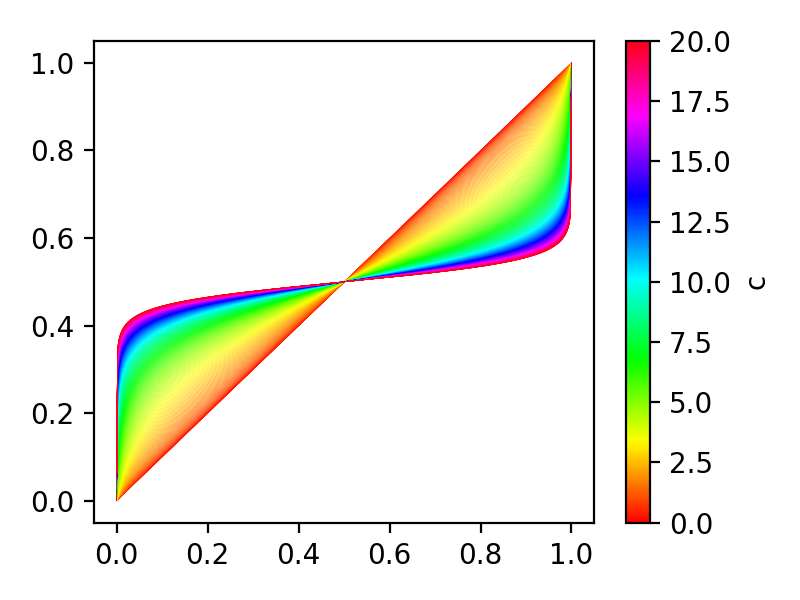
\includegraphics[width=\linewidth]{img/s_curve_c.png}

  \subcaption{Sampling $S^-1(x)$ with $r \cdot N$ samples for $\left[S(-c), S(0)\right]$ and $(1-r) \cdot N$ samples for $\left[S(0), S(c)\right]$}
  \label{fig:s_curve_r}
  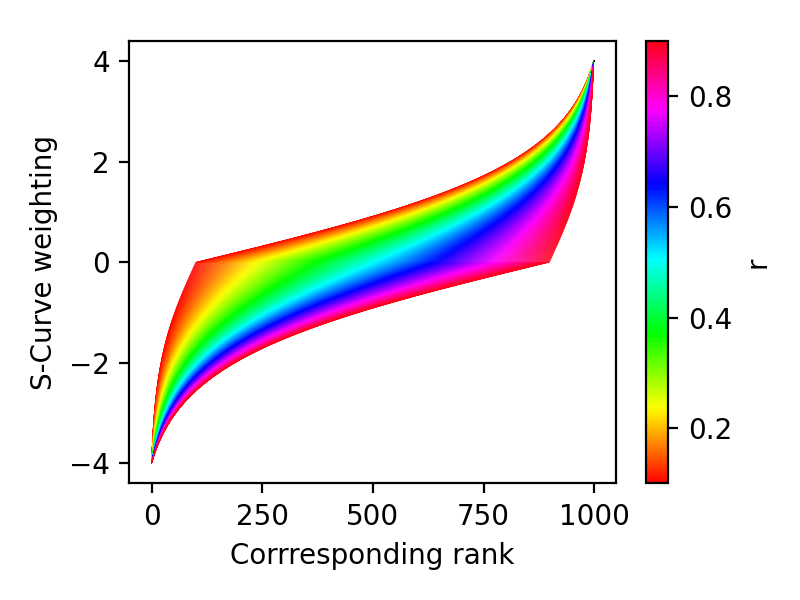
\includegraphics[width=\linewidth]{img/s_curve_r.png}
\end{figure}

To apply the soft-veto, each score in the rank list is multiplied by the s-curve correspond rank.
This soft-veto methodology can be used on certain rank list before fusing, to have a more cleaved decision on the link nature.

\subsection{Authors Clustering}

To find clusters of authors, a possible way is to use a hierarchical clustering algorithm on a rank list.
In a rank list, at each rank the link indicate if the two documents should belong to the same cluster in order of certainty.
The hardest task in this clustering scheme is to find where the list should be cutted, such that the number of true links above the cut is maximized and the number of false links under the cut is minimized.
To find this cut, two apporaches were explored : one using a unsupervised clustering evaluation technique which is totaly unsupervised and another one using a linear model to learn to make this cut but it requires a training dataset.

\subsubsection{Agglomerative clustering}

The scikit-learn package~\cite{sklearn} provide an implementation bottom-up implementation of the hierarchical clustering, which is usually called agglomerative clustering.
Using this approach, at the start of the algorithm, each document belong to a different cluster.
Clusters are merge based on the scores in the rank list, each step the algorithm merge clusters using the minimal score based on the linkage criteria.
Multiple linkage criteria are available : \textit{ward} (metric that aim to minimize the variance of the cluster merged), \textit{average-linkage} (use the average score of each links of the cluster merged), \textit{complete-linkage} (use the maximal score of the cluster merged), \textit{single-linkage} (use the minimal score of the cluster merged).
Ward linkage was discarded since the implementation only allow euclidean distance for its computation.
Since the number of clusters is unknown, the merging procedure is stopped based on a maximal threshold.
In this study the optimal threshold is found using two approach, one in an unsupervised way and another one in a supervised way.

\subsubsection{Learning the threshold in a unsupervised way}

The idea is to run the agglomerative clustering on multiple time and stop at each number of clusters.
This produce $N$ possible clusterings, each of those can be evaluated using the silhouette score.
See definition~\ref{def:silhouette}.

\begin{definition}[Silhouette score~\cite{sklearn}]
  \label{def:silhouette}
  The silhouette score is a unsupervised clustering metric which evaluate a clustering result by measureing the cohesion and separation of the clusters.
  \begin{equation}
    \frac{b - a}{max(a, b)}
  \end{equation}
  \begin{equation*}
    \begin{split}
      a&: \text{intra-cluster distance}\\
      b&: \text{nearest-cluster distance}
    \end{split}
  \end{equation*}
  The value is ranged between -1 and 1, a large value indicate a good cohesion and good separation of the clusters (low intra-cluster distance, high nearest-cluster distance).
\end{definition}

When iterating over the number of clusters each times the median silhouette score for each cluster is computed.
When this score reach below 0, the last positive score clusters is kept.
If the procedure does not reach a score below 0, the maximal is kept.
This procedure is called Iterative Positive Silhouette (IPS) and was proposed in~\cite{automated_unsupervised}.

\subsubsection{Learning the threshold in a supervised way}

To learn at which position in the rank list the cut should be, this second idea is to fit a linear model on samples created with the rank list.
To train the model, a sample is created for each link in a rank list.
The links labels are either \textit{true} when both document in the link are from the same author and \textit{false} otherwise.
The features used are : the log of the relative rank ($log(\frac{rank}{|L|})$ and the score of the link.
Since the training is only based on the relative rank and the score at each rank, the trained model is language independent and size independent.
But this model is metric dependent, since the score is not normalized.

In this study the model used is the logistic regression.
To find the cut on the test datasets, the fitted model is used on every links in the testing rank list, the number of \textit{true} labels give the rank at which the last link should be merged.
The links are labeled as \textit{true}, when the probability of being a true link is greater than $0.5$.
This model can be used on any other rank lists produced with the same distance metrics.
Using agglomerative clustering the maximal distance threshold is the score of the last link to merged.

\subsection{Pipeline}

Most of the methods presented in this section can be combined in the process. This process is synthesized in Figure~\ref{fig:pipeline}

\onecolumn
\begin{figure}[p]
  \centering
  \caption{Pipeline}
  \label{fig:pipeline}
  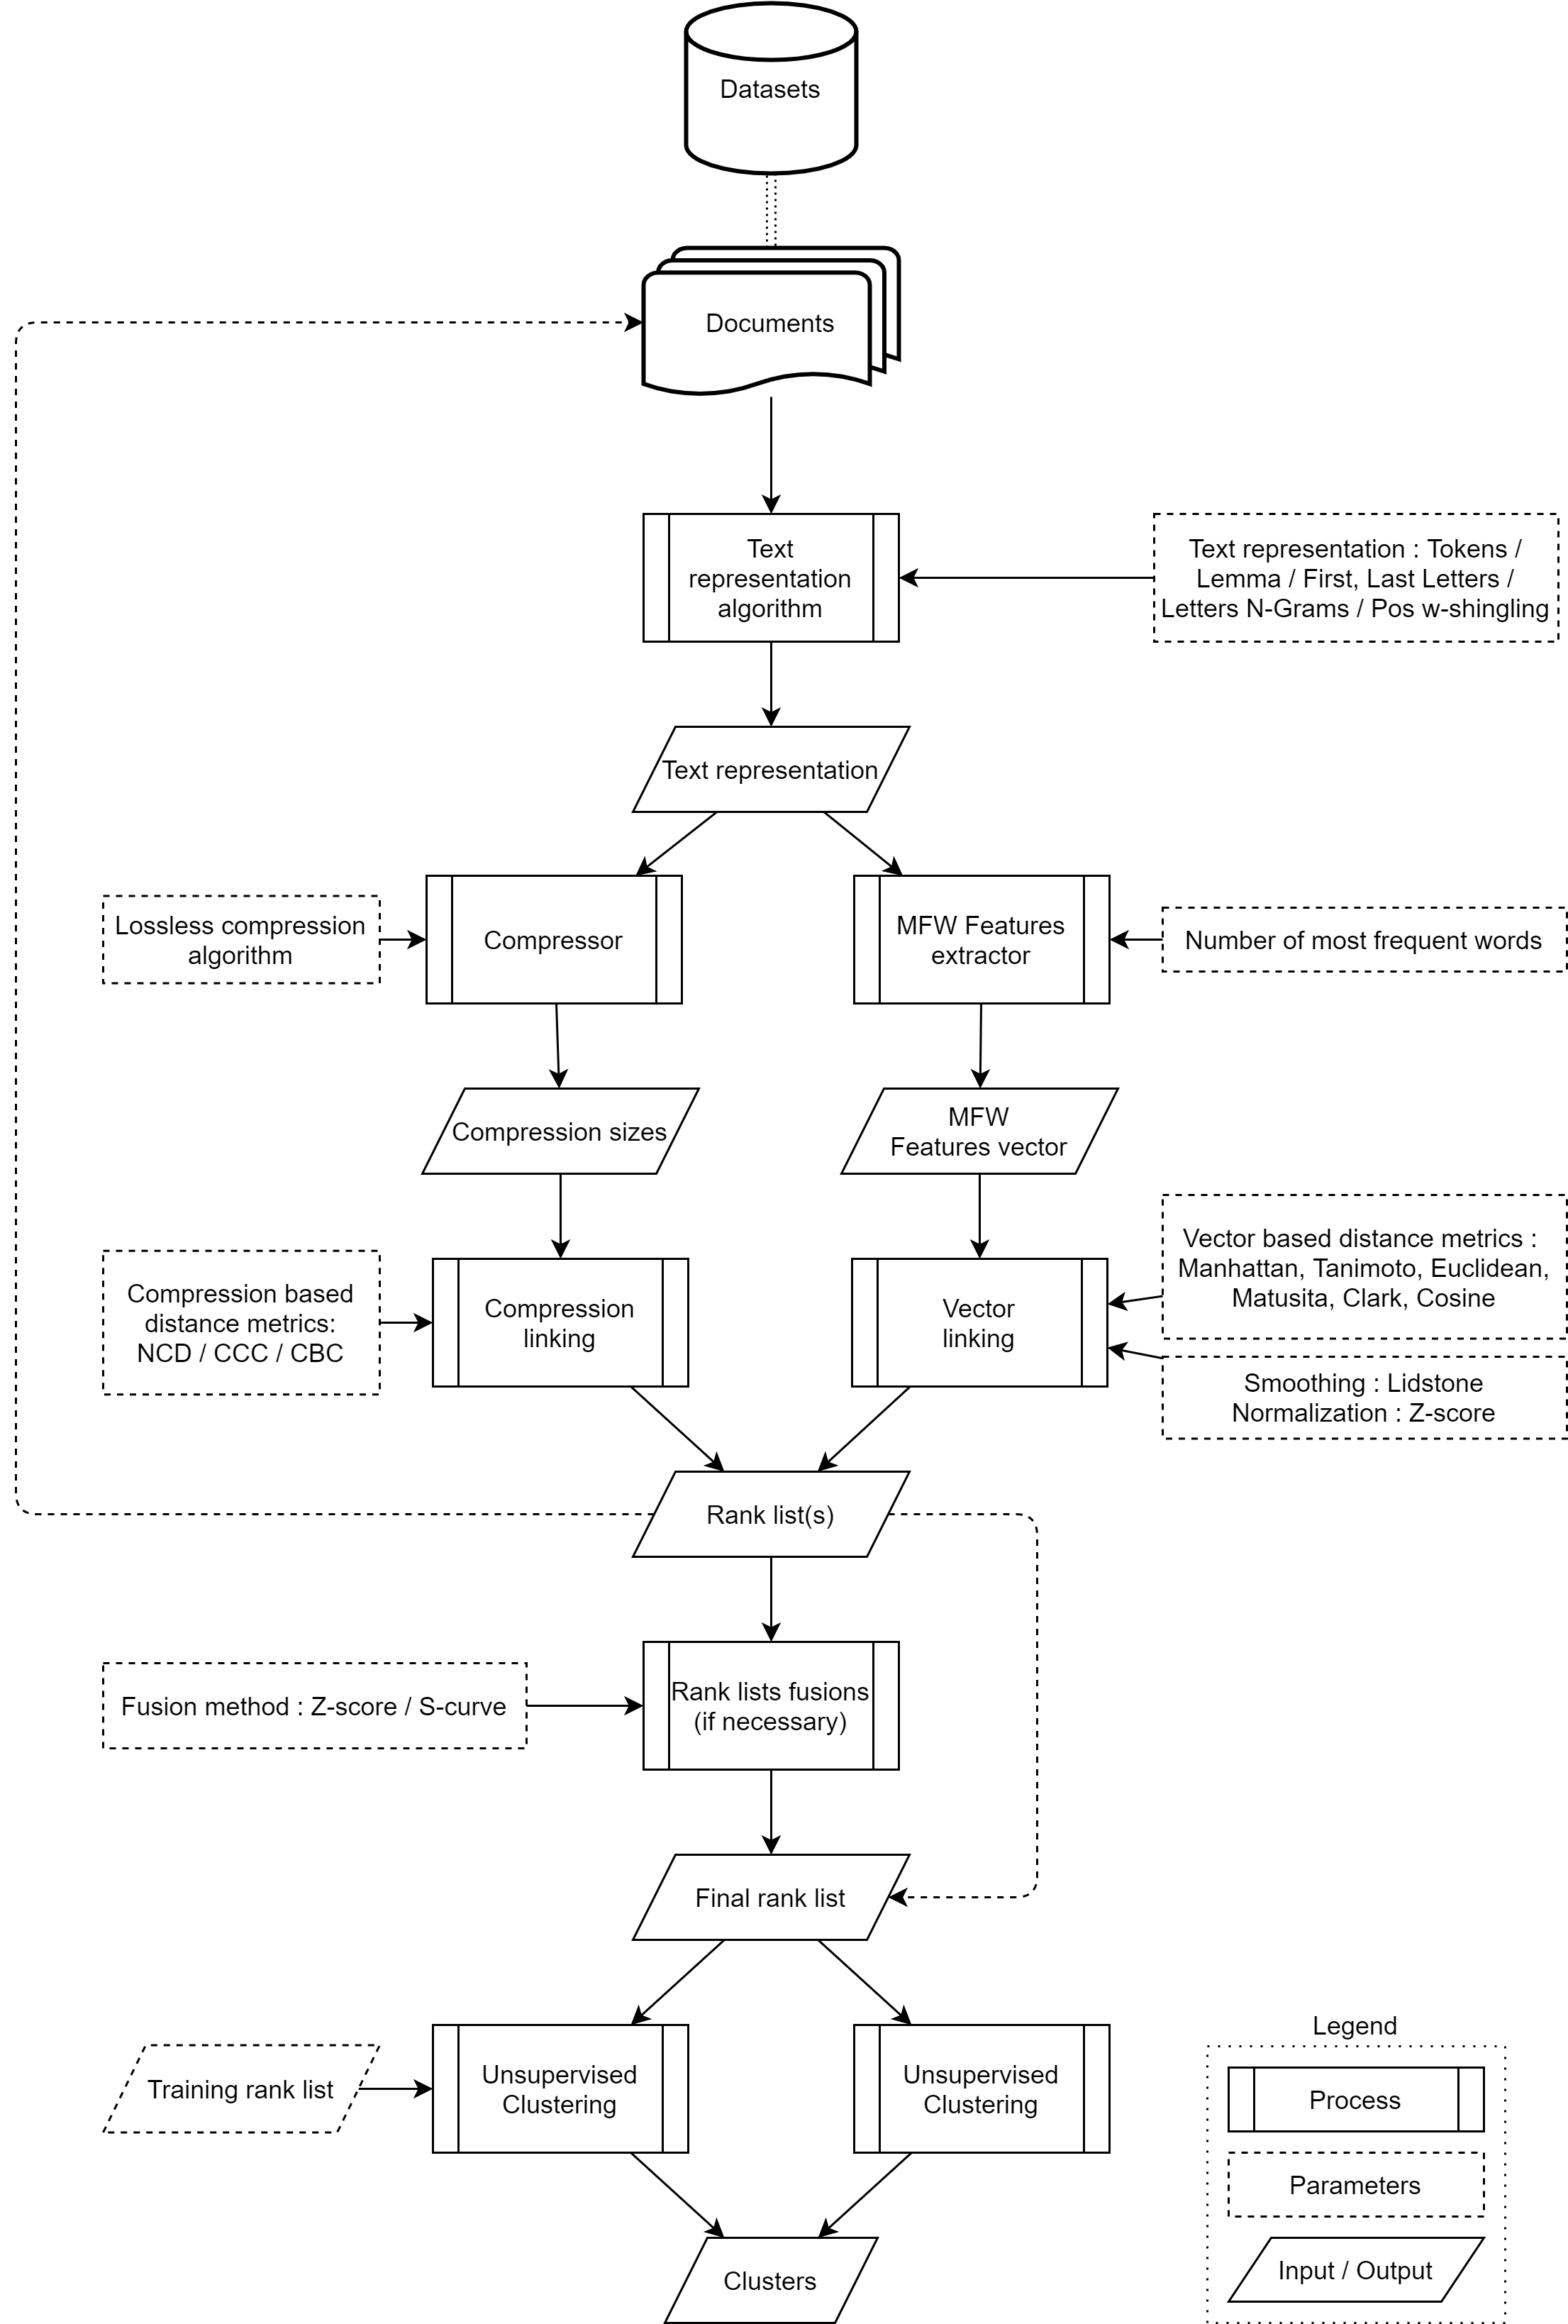
\includegraphics[width=\textwidth,height=\textheight,keepaspectratio]{img/pipeline.png}
\end{figure}
\twocolumn
